\documentclass{article}
\usepackage{amsmath}
\usepackage[ngerman]{babel}
\usepackage[utf8]{inputenc}
\usepackage{anysize}
\usepackage{fancyhdr}
\usepackage{graphicx}

\parindent0em
\graphicspath{figures/}


\pagestyle{fancy}
\fancyhf{}
\fancyhead[C]{Collector's Edition -- Technical Rider}
\fancyfoot[LE,LO]{collectorseditiontheband@gmail.com}
\fancyfoot[RE,RO]{+49 176 609 622 87}

\title{
\includegraphics[width=0.4\textwidth]{figures/BandLogo} \\Tech Rider}
\date{Letzte Änderung am \today}

\begin{document}

  \maketitle
  \thispagestyle{empty}

  \section*{Allgemeines}
  Mit diesem Rider könnt ihr euch vorab ein Bild von unseren technischen Vorstellungen machen.
   Er soll uns allen die Durchführung erleichtern. Wir wissen, dass es fast unmöglich ist, alles so
   perfekt hinzubekommen, wie wir es haben möchten. Dafür haben wir Verständnis und würden uns über eine
   Kontaktaufnahme freuen, um Abweichungen besprechen zu können. Es ist uns wichtig, dass alle Parteien
   vernünftig informiert sind damit alles reibungslos und vor allem mit viel Spaß ablaufen kann.

   Bei technischen Fragen wenden sie sich bitte per Mail an uns.\\
   collectorseditiontheband@gmail.com\\
   Vielen Dank!

  \section*{PA-System}

  Eine zur Location passende PA \& Lichtanlage muss Seitens des Veranstalters gestellt und supported
  werden. Es wird vorausgesetzt, dass die Bühne, PA und Lichttechnik vor dem Eintreffen der Band fertig
  aufgebaut, getestet und voll funktionsfähig ist. Um die Sicherheit der Musiker, Crew und des Publikums
  nicht zu gefährden garantiert der Veranstalter die Einhaltung der geltenden Sicherheits- und
  Unfallverhütungsbestimmungen, insbesondere der Normen VDE und BGV. Dieser Technical Rider ist
  Bestandteil des Gastspielvertrags.

  \section*{Backline}

  Collector's Edition bringt typischerweise keine Backline mit. Somit wird folgendes
  benötigt:

  \begin{enumerate}
  \item Ein Drumset inkl. Teppich (idealerweise außerdem ein Drumriser) mit
  mindestens 2 Hängetoms, einer Floortom, 3 Cymbal Stands, HiHat und Snare Stand.
  \item Ein Bassamp (vorzugsweise 4x10", 8 Ohm)
  \item Zwei 2x12" Gitarrenamps (vorzugsweise Vox AC30 C2)
  \item Vier Mikrofone inkl. Ständer (vorzugsweise Shure SM58)
  \end{enumerate}

  \section*{Bühne}

  \underline{Collector's Edition reist ohne eigene Techniker}

  Bei Eintreffen von Collector's Edition muss die B\"uhne gereinigt und bezugsfertig sein.
  Bei Open-Air-Veranstaltungen muss die Bühne zudem auch durch Dach- und Wände sowie
  durch flachen, ebenen Bühnenboden ordentlich vor Witterung geschützt sein.

  Ein Riser (2m x 2m x 0,4m) für das Schlagzeug, mittig an der Bühnenhinterkante, muss aufgebaut
  sein.


  Wir freuen uns über einen kompetenten, netten, nüchternen und ausgeschlafenen Tontechniker, der
  mit der elektrischen Anlage vertraut ist, der vom Get-in bis zum Ende der Veranstaltung für technische
  Fragen Ansprechpartner ist.

  \section*{Monitoring}

  Auf der Bühne benötigen wir:\\
  3 Wedges + 1 Drumfill\\

  \begin{tabular}{l l}
  Mix 1 - E Gitarre (StageRight / 1 Wedge) & Mix 3 - Bass (StageLeft / 1 Wedge) \\
  Mix 2 - E Gitarre (Center / 1 Wedge)     & Mix 4 - Drums (Drums / 1 Drumfill) \\
  \end{tabular}

  \section*{Mischpult}
  Das Mischpult sollte über mindestens 24 freie Kanäle und vollparametrische EQs verfügen.

  \section*{Channellist}

  \begin{tabular}{|l|l|l|l|l|}
  \hline
  \textbf{Kanal} & \textbf{Instrument} & \textbf{Mic (Vorschläge)} & \textbf{Stativ} & \textbf{48V}\\
  \hline
  1  & Kick           & Audix D6/ D70d             & Small Boom &   \\
  2  & Snare Top      & Audix D1 / D58c            & Clip       &   \\
  3  & Snare Bottom   & SM 57                      & Clip       &   \\
  4  & HiHat          & KM 185 / MC 950            & Small Boom & X \\
  5  & Tom1           & Audix D2 / D58c            & Clip       &   \\
  6  & Tom2           & Audix D2 / D58c            & Clip       &   \\
  7  & FloorTom       & Audix D4 / D57c            & Clip       &   \\
  8  & OH L           & KM 184 / MC 930            & Tall Boom  & X \\
  9  & OH R           & KM 184 / MC 930            & Tall Boom  & X \\
  10 & Bass DI Passiv & -                          & --         &   \\
  11 & Git1 Mic       & SM 57                      & Small Boom &   \\
  12 & Git2 Mic       & SM 57                      & Small Boom &   \\
  13 & Voc1           & SM 58                      & Tall Boom  &   \\
  14 & Voc2           & SM 58                      & Tall Boom  &   \\
  15 & BackVoc1       & SM 58                      & Tall Boom  &   \\
  16 & BackVoc2       & SM 58                      & Tall Boom  &   \\
  17 & AtmoL          & KM 184 / Rode NT5 / MC 930 & Small Boom & X \\
  18 & AtmoR          & KM 184 / Rode NT5 / MC 930 & Small Boom & X \\
  \hline
  \end{tabular}

  \section*{Stage Plan}

  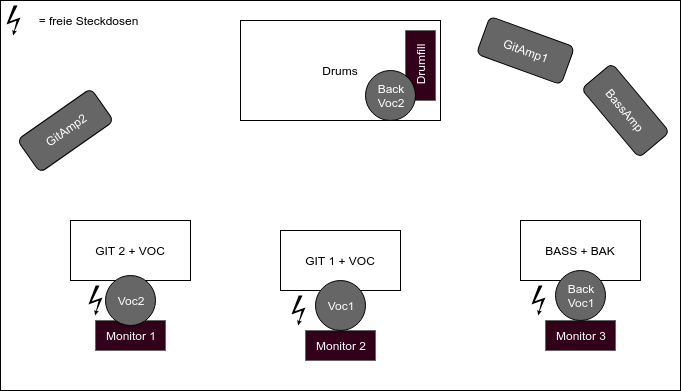
\includegraphics[width=\textwidth]{figures/StagePlan}


\end{document}
